\chapter{Background and Overview of End to End Modeling Methods}

\section{Chapter Abstract}

This chapter presents the methods used to identify the scope of this dissertation's research around the total costs of ownership of data centers. These are the methods used to understand and address the scope of a succinct research questions that seek to address total costs of building infrastructure of hyper-scale internet data centers. It begins by describing data centers based on past literature to set the context of the research undertaking. Then the chapter discusses the resulting modeling framework from the culmination of the literature reviews and the researcher's professional experiences. The presented model is capable of quantifying the end to end costs of a the global system using life cycle analysis frameworks by demonstrating its effectiveness with the quantification of $CO_2$ emissions. 

\section{Introduction}

    This research considers energy and $CO_2$ inventories across the life time of hyper-scale data centers (DC). These DCs house scalable computational architectures consisting of buildings, cooling plants, power distribution systems, compute hardware, digital storage hardware, and network hardware which are the status-quo for internet service operations. Physically, the size of individual internet DC facilities have increased from modest footprints to now span millions of square feet over the last decade; coinciding with ubiquitous penetration of the internet into the lives of people around the world . The increase in demand for DCs motivates this work as a tool kit in the DC building infrastructure design process. Beyond, the building design process, this kit is intended to be an element for broader business models for internet products.
    
    For internet products, DCs represent a major fraction of their total costs of operations and environmental footprints.  This work develops a modeling framework that couples building energy models, marginal cost of grid energy models, and the embodied costs of materials to provide an end to end assessment of data centers. Specifically, this dissertation demonstrates the models by quantifying the $CO_2$ emissions as a singular metric that is is sufficiently analogous monetary costs.
    
    In the next section, some background and past literature about the sustainability of data centers is presented first. The background indicates the research motivation behind the life cycle perspective for data center systems. Then second, seminal works that have analyzed data center life cycle costs are reviewed. These works guide the development of resulting model from this research by pointing to low hanging fruits and gaps in the current practices. They are the inspiration of the research's methodology. Ultimately, this chapter provides an overview of the technical problem space and it points to past works that inspire the solution methods.

\section{Background}

    Data centers (DCs) will consume 13\% of the worlds energy production by 2030 according to worst case prediction models \cite{andrae15}. This high energy demand is not surprising given the ubiquitous penetration of the internet nowadays. For internet DC infrastructure, the energy demand problem space is compounded by a rapid pace of hardware technology innovations on one hand. On the other hand, factoring software technology innovations lead to models that show a brighter picture. This picture is aligned with current trends, where efficiency across the entire DC stack indicates a downward trend for power demand per unit of performance. As an example, by 2016 performance throughput had increased 350\% since 2012, relative to the power demand for computer hardware \cite{GoogleEnvRpt}.  The hardware efficiency gains seen over the last decade still do not offset the need for additional DC physical capacity.
    
    Internet DC capacity is not bound by physical sizes or geographic locations however. Location agnostic networks spanning the globe allow information technology (IT) systems to scale in resource parameters such as CPU, GPU, memory, storage, and data access rates. Parametric scaling of these resources enables operational tuning to compensate for physical capacity constraints. Capacity fungibility of DC parameters at a global scale leads businesses with risky practices to provision building scale data-center infrastructure very lean. While businesses that are adverse to risk can be excessively conservative. In the case of lean provisioning, all physical resources are highly utilized with little or no headroom. For the conservative approaches, normal operating conditions are such that sustained operational points are well below the capacity of the equipment. Operations significantly below capacity allows the service to accept bursts in service, inorganic  growth, and be fault tolerant in case of failures elsewhere in the system. 
    
    Lean and conservative operations are both classified as equivalent based on today's sustainability indicators and both have strategic advantages for data center owners. For example the abrupt change in internet traffic for many communications, media, and collaboration web sites due to COVID have critical dependencies on data center facilities. These change in traffic pattern are shown in Figure~\ref{img_nyt_covid}, if the data centers were operational loaded to peak capacity then it would be impossible to absorb such drastic changes.
    
    \begin{figure} [!h]
\centering
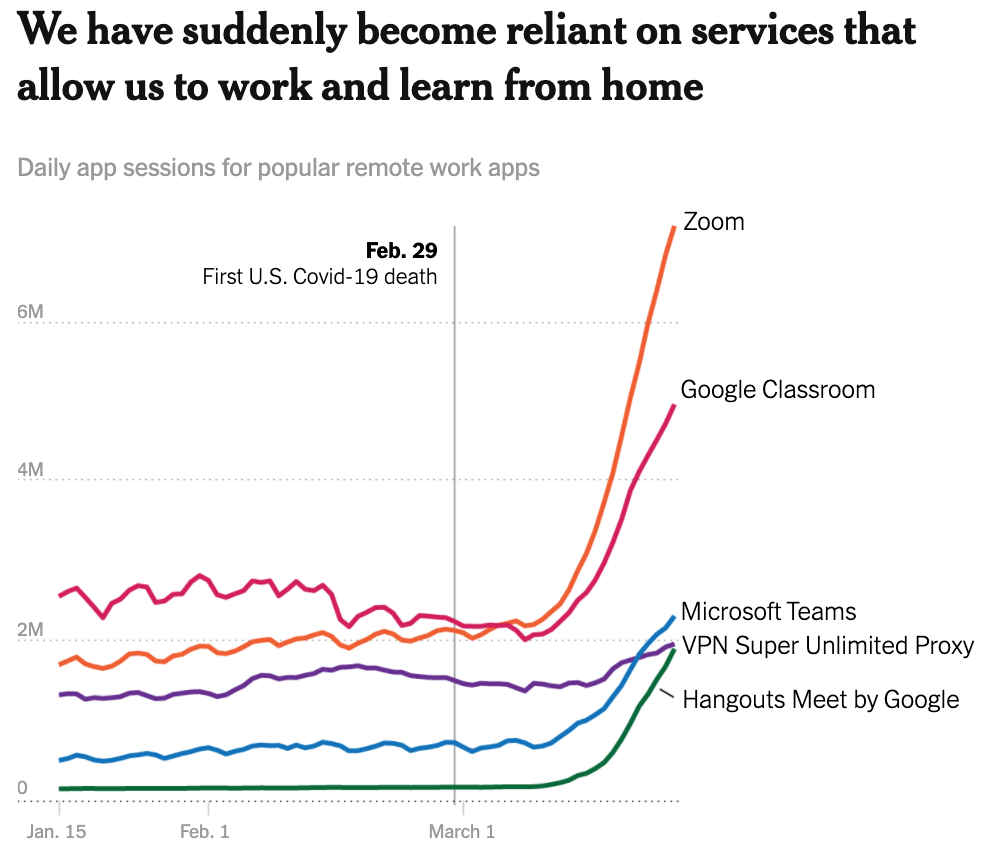
\includegraphics[scale=.3]{methodology/images/nyt_covid_internet.png}
\caption[Internet Traffic Change due to COVID]{Internet Traffic Change.  Image from \cite{nyt_corna_virus}}
\label{img_nyt_covid}
\end{figure}
    
    Furthermore, DC facilities can be measured with multiple attributes; power limits, cooling limits, network limits, and floor space. Where power has shown to be the most prevalent indicator of DC, \cite{barroso18}. However, the other attributes don't linearly scale with power. For example, the researcher designed a data center in mid 2013 based on historical trends. By the time the data center was deployment the power density per information technology devices had significantly increased. With the increase in the power density, more that 60\% of the designed floor space was left stranded (ie not deploy-able as the facility was power and cooling limited at 40\% of the designed area). However, if the DC design team had looked closer at Moore's law such disruptive change in density were apparent. Figure~\ref{img_moores} indicates the log-scale nature of de-materialization of transistor based technology made famous by Moore.
    
    \begin{figure} [!h]
\centering
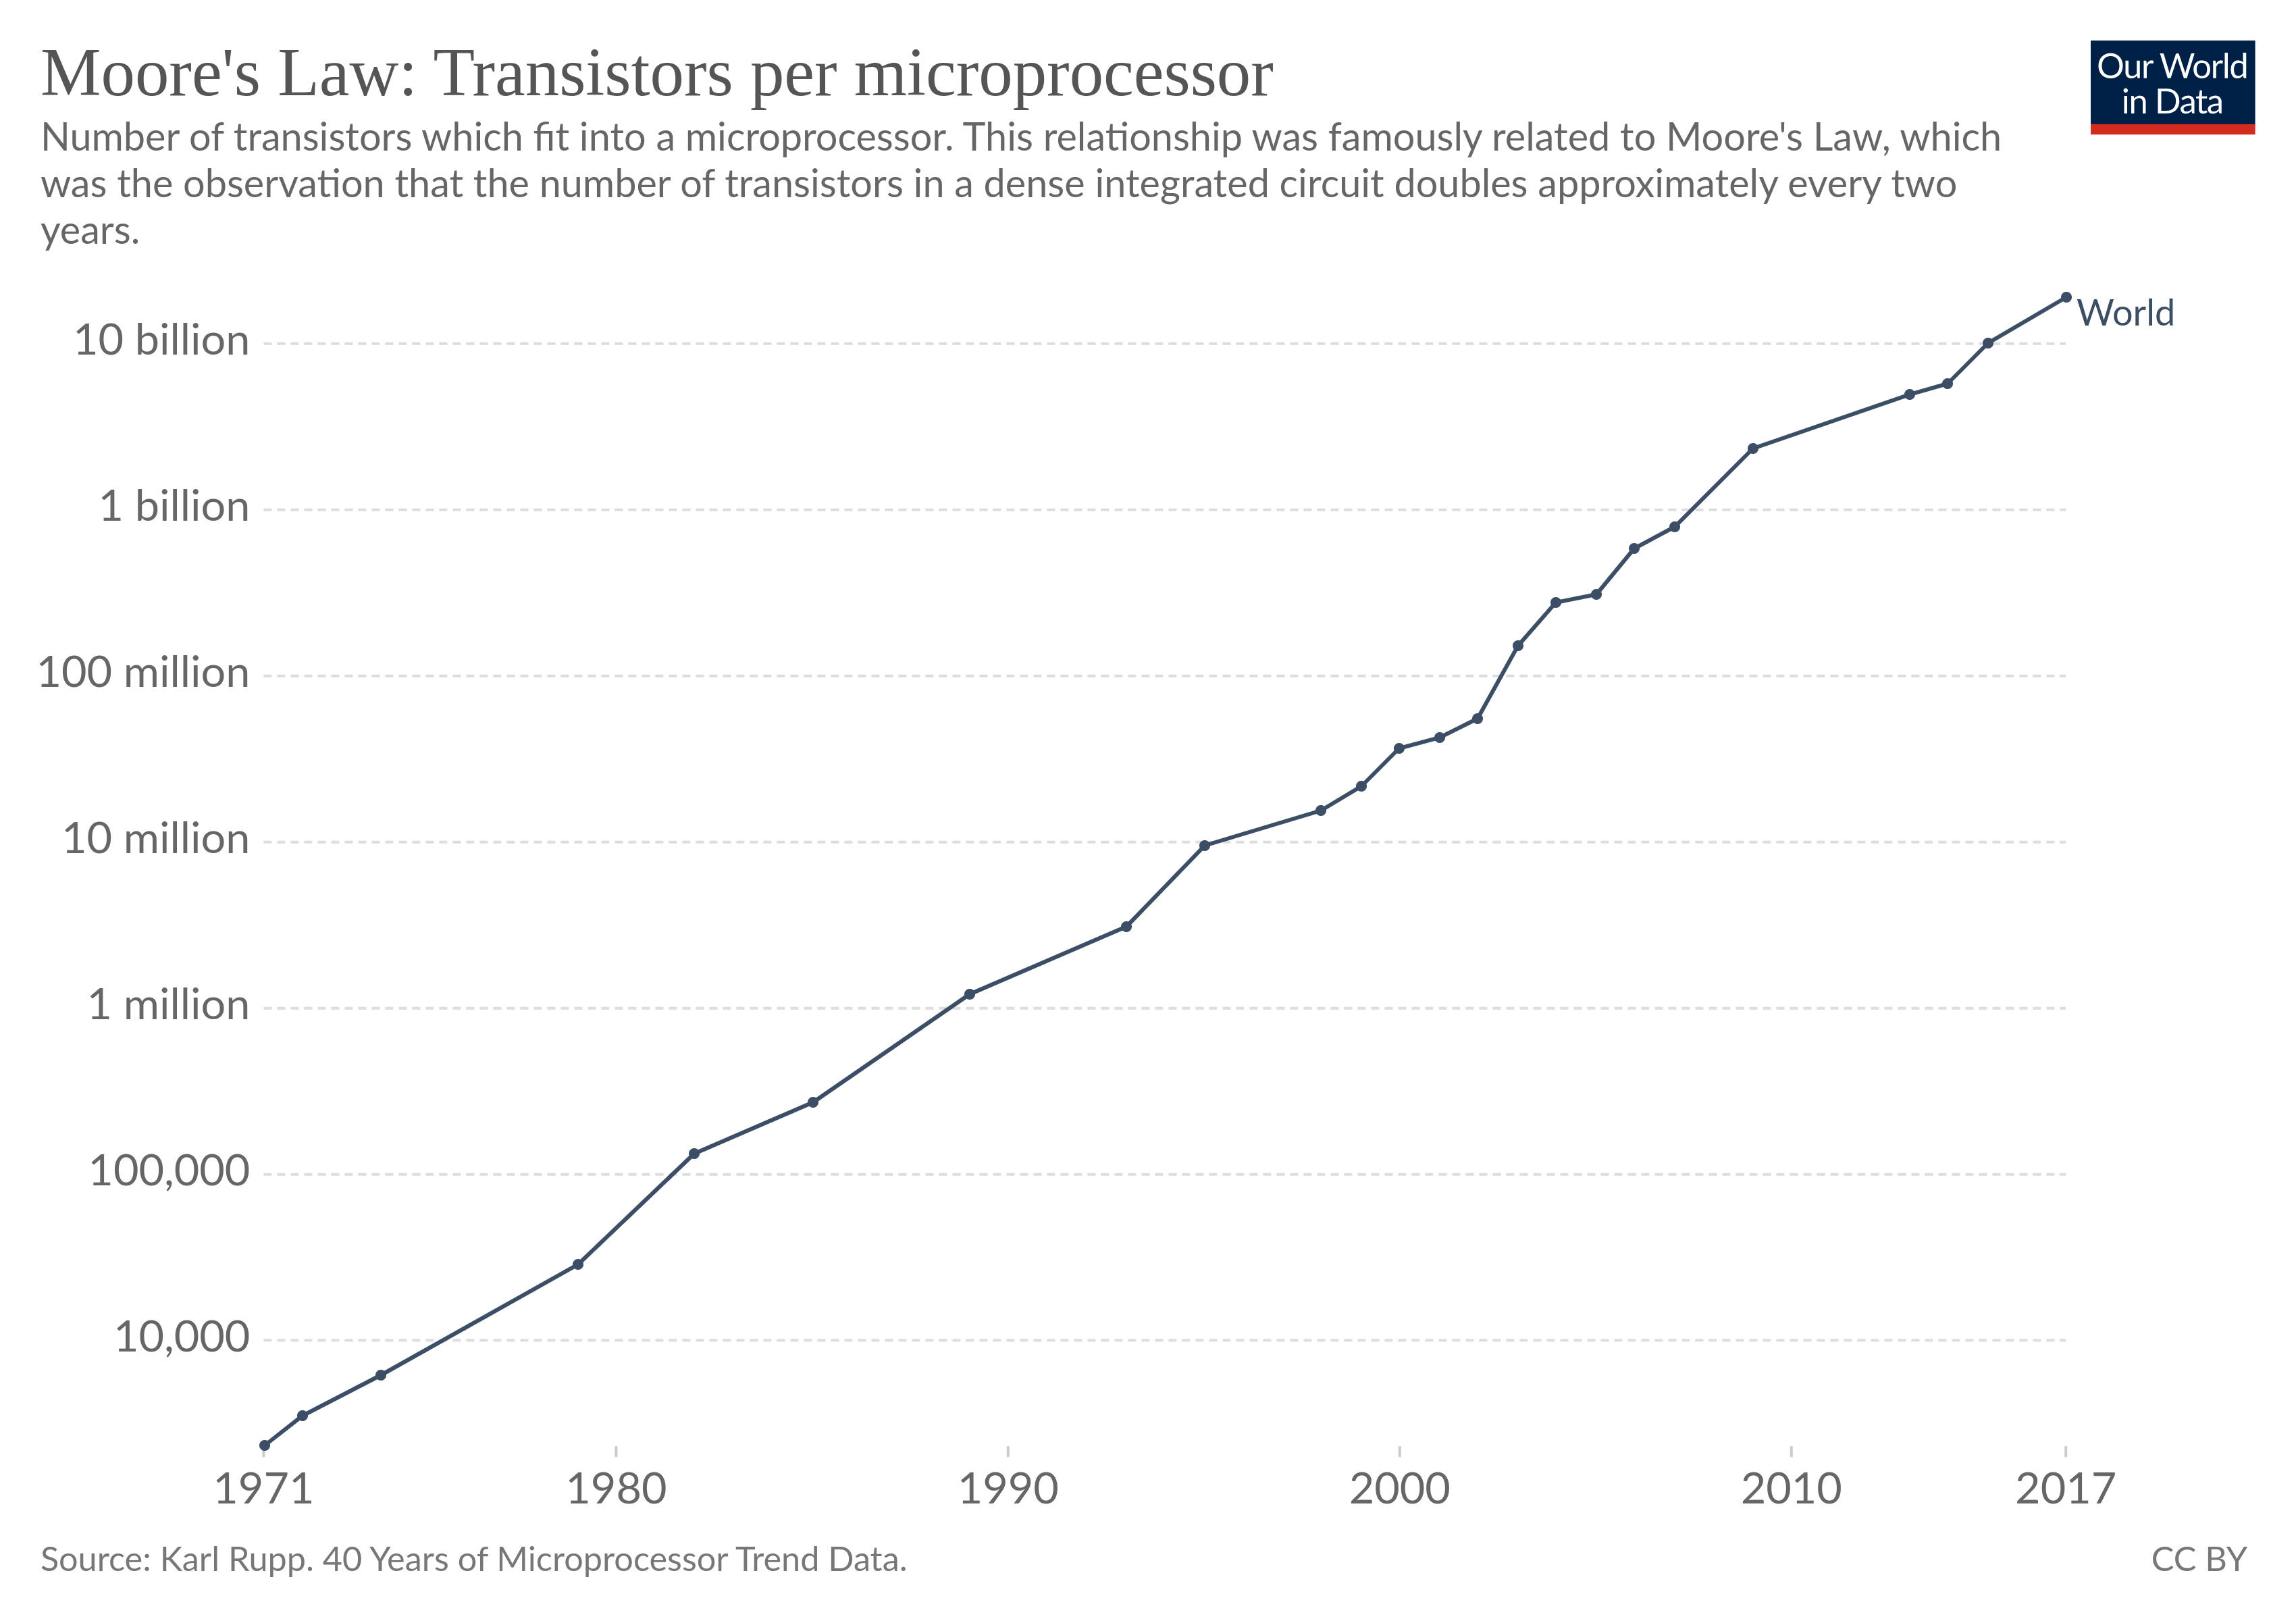
\includegraphics[scale=.1]{methodology/images/transistors-per-microprocessor.png}
\caption[Moore's Law]{Moore's Law: Transistors per microprocessor.  Image from \cite{world_data}}
\label{img_moores}
\end{figure}
    
    The prevalent indicator for sustainability of DC facilities is currently the Power Usage Effectiveness metric ($PUE$, see equation \ref{eq:pue}). $PUE$ is a dimensionless ratio of load vs. supply energy.   In the equation $E_{IT}$ indicates the IT energy load and $E_{total}$ indicates the total energy supplied to the facility. The $PUE$ is generally reported in a quarterly or annual basis by integrating the equation across the respective time period. For a given period, the metric measures the operational efficiency of the facility's system compared to the information technology equipment (ITE). Spaces housing ITE have seen profound cooling and power distribution efficiency gains resulting from the focus on $PUE$, however the metric does not comprehensively cover sustainability of DCs.
    
    \begin{equation} \label{eq:pue}
    PUE=\frac{E_{total}}{E_{IT}} 
    \end{equation}
    
    The $PUE$'s shortcomings as a sustainability metric are noted by Horner, particularly that low PUEs do not correlate to low carbon footprint \cite{Horner16a}. The tendency of carbon intensity to vary based on energy source characteristics is demonstrated by Masanet in \cite{Masanet13a}. Masanet shows that energy supply sources must be coupled with lowered demands to be good indicators of use phase carbon footprint. For example, the carbon footprint of a low $PUE$ DC with it's energy sourced from a coal plant will be higher compared to a DC that operates with a slightly higher $PUE$ but sources power from a renewable source. This is summarized in Figure~\ref{masanet13a1}.
    
    \begin{figure} [!h]
\centering
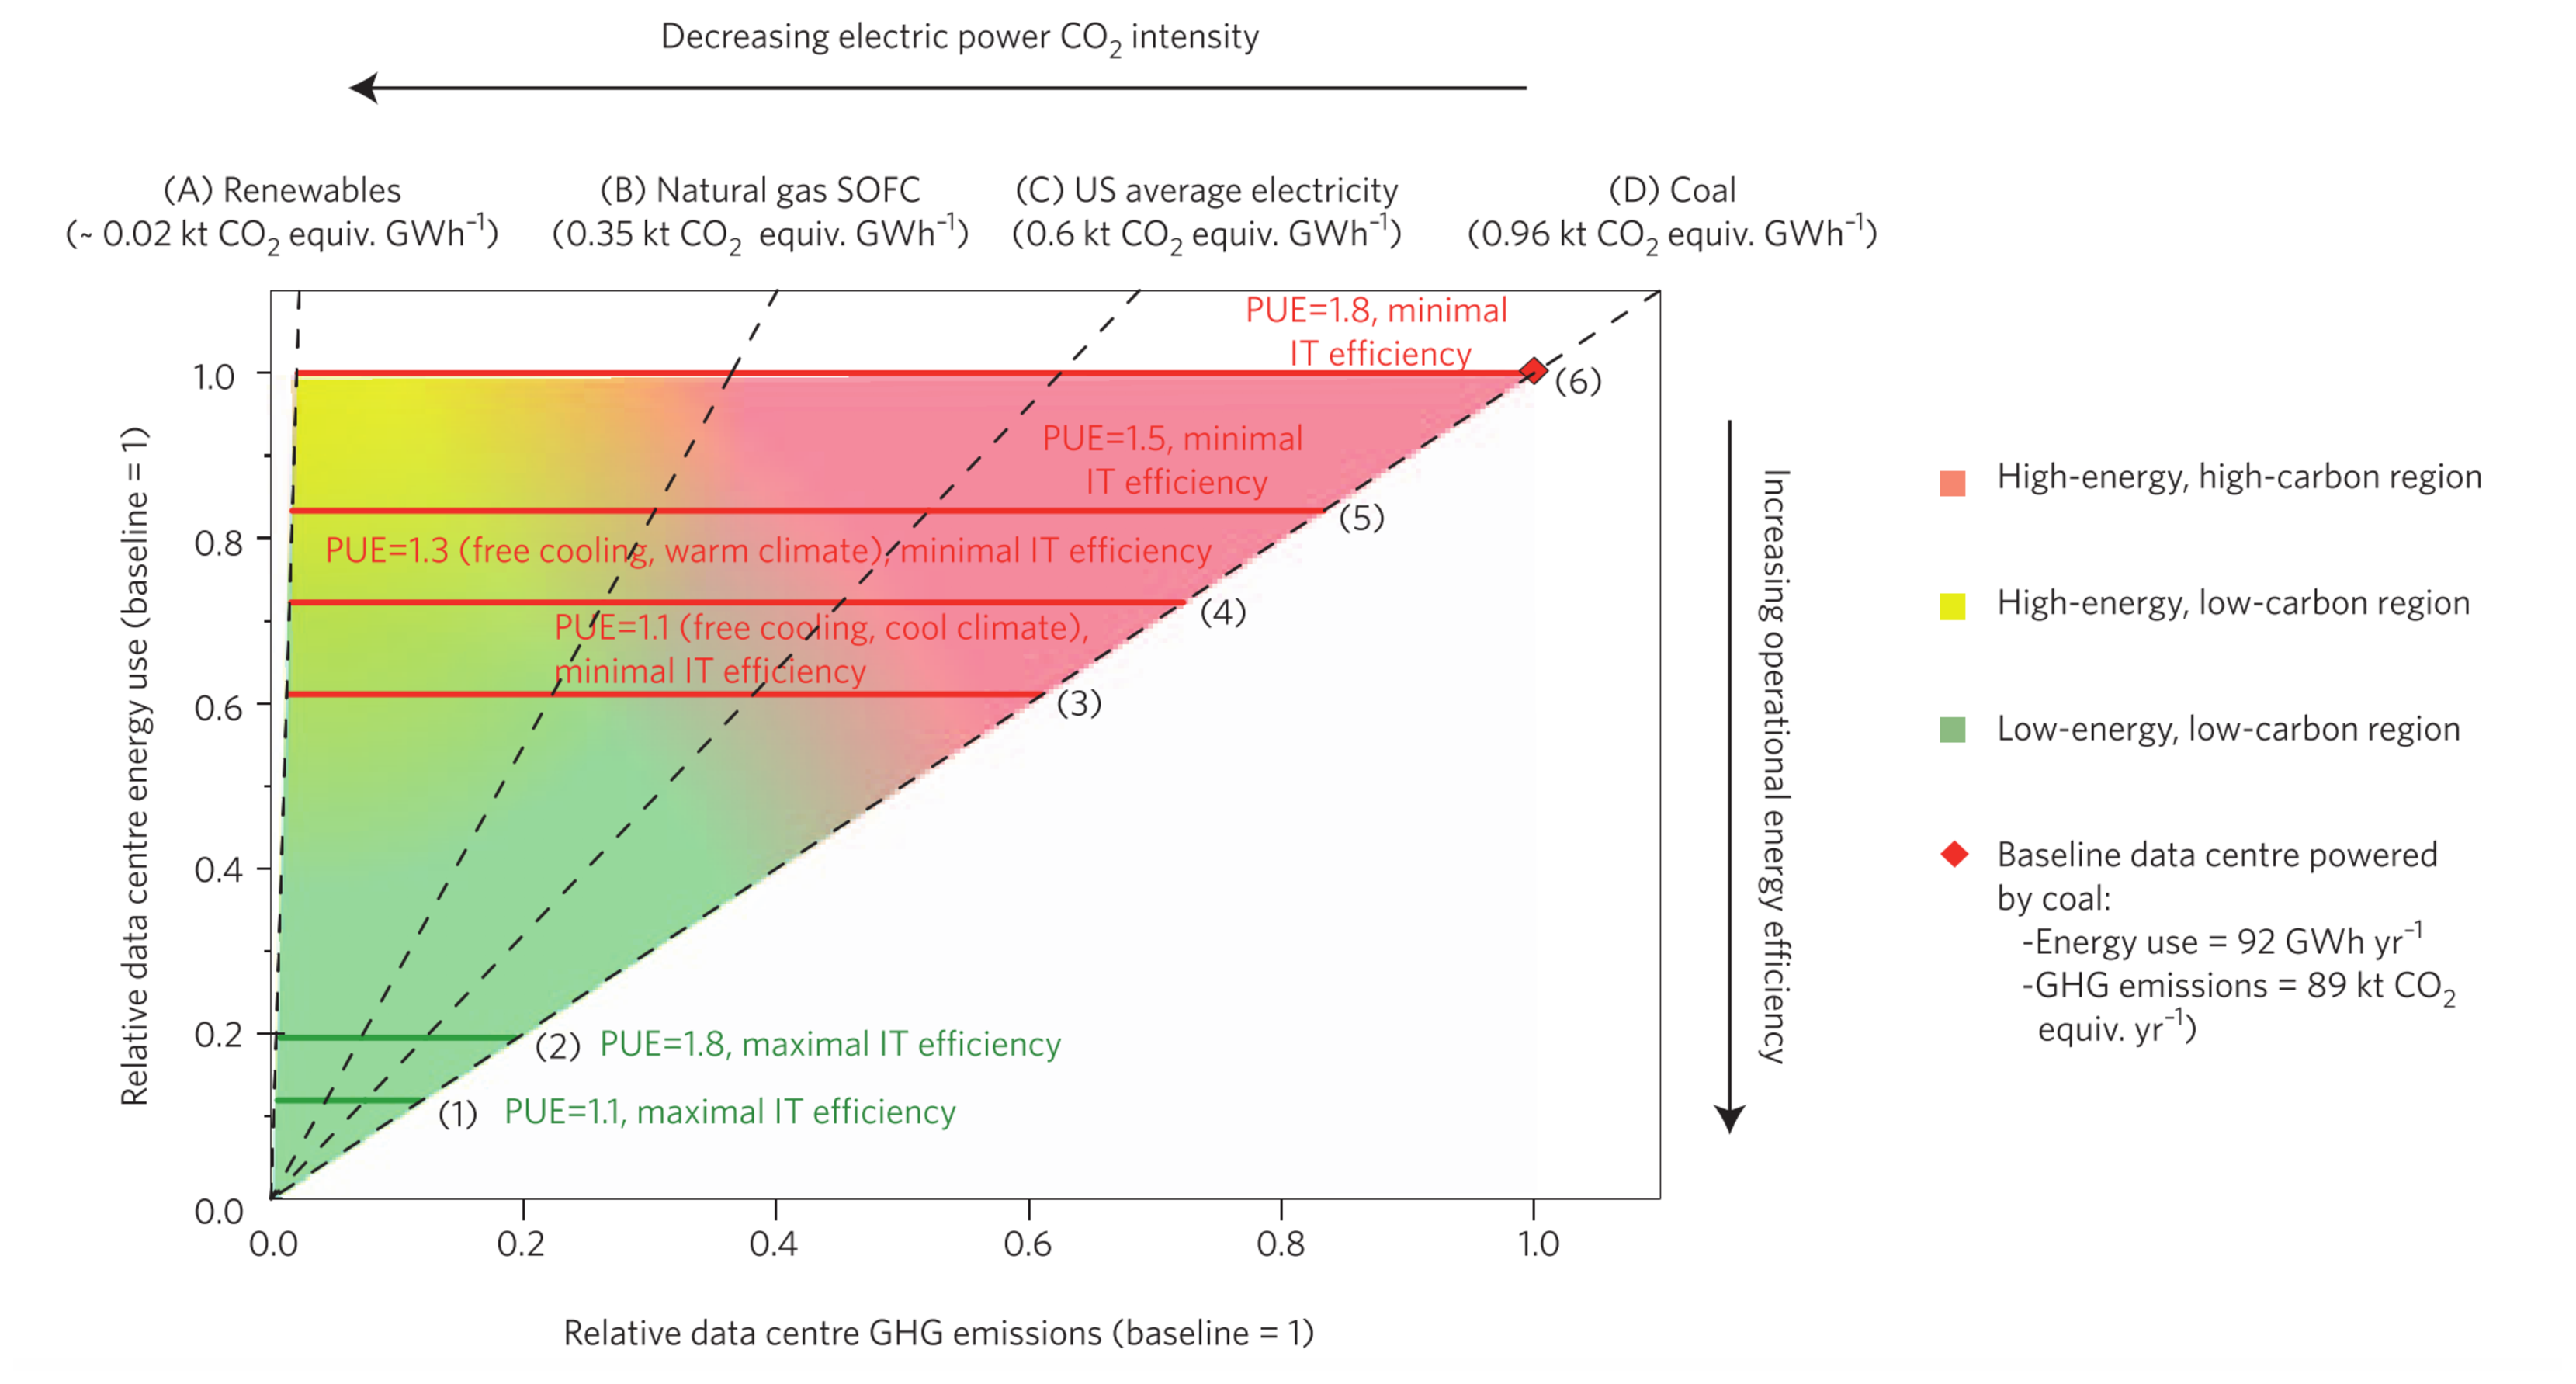
\includegraphics[scale=.25]{methodology/images/masanet13a1.eps}
\caption[Energy Use vs. Carbon performance map]{Energy Use vs. Carbon performance map. Image from \cite{Masanet13a}}
\label{masanet13a1}
\end{figure}
    
    With the proliferation of the PUE as the de-facto efficiency metric, ASHRAE recognized the significance of the cooling systems to the data center energy use. In rapid response they began to develop guidelines to help operators optimize their cooling systems. One of the most profound contribution from ASHRAE has been their position on expanded thermal window for the data center environments. The expanded thermal window has an influence nearly all elements of a data center facility. 
    
    \begin{figure} [!h]
\centering
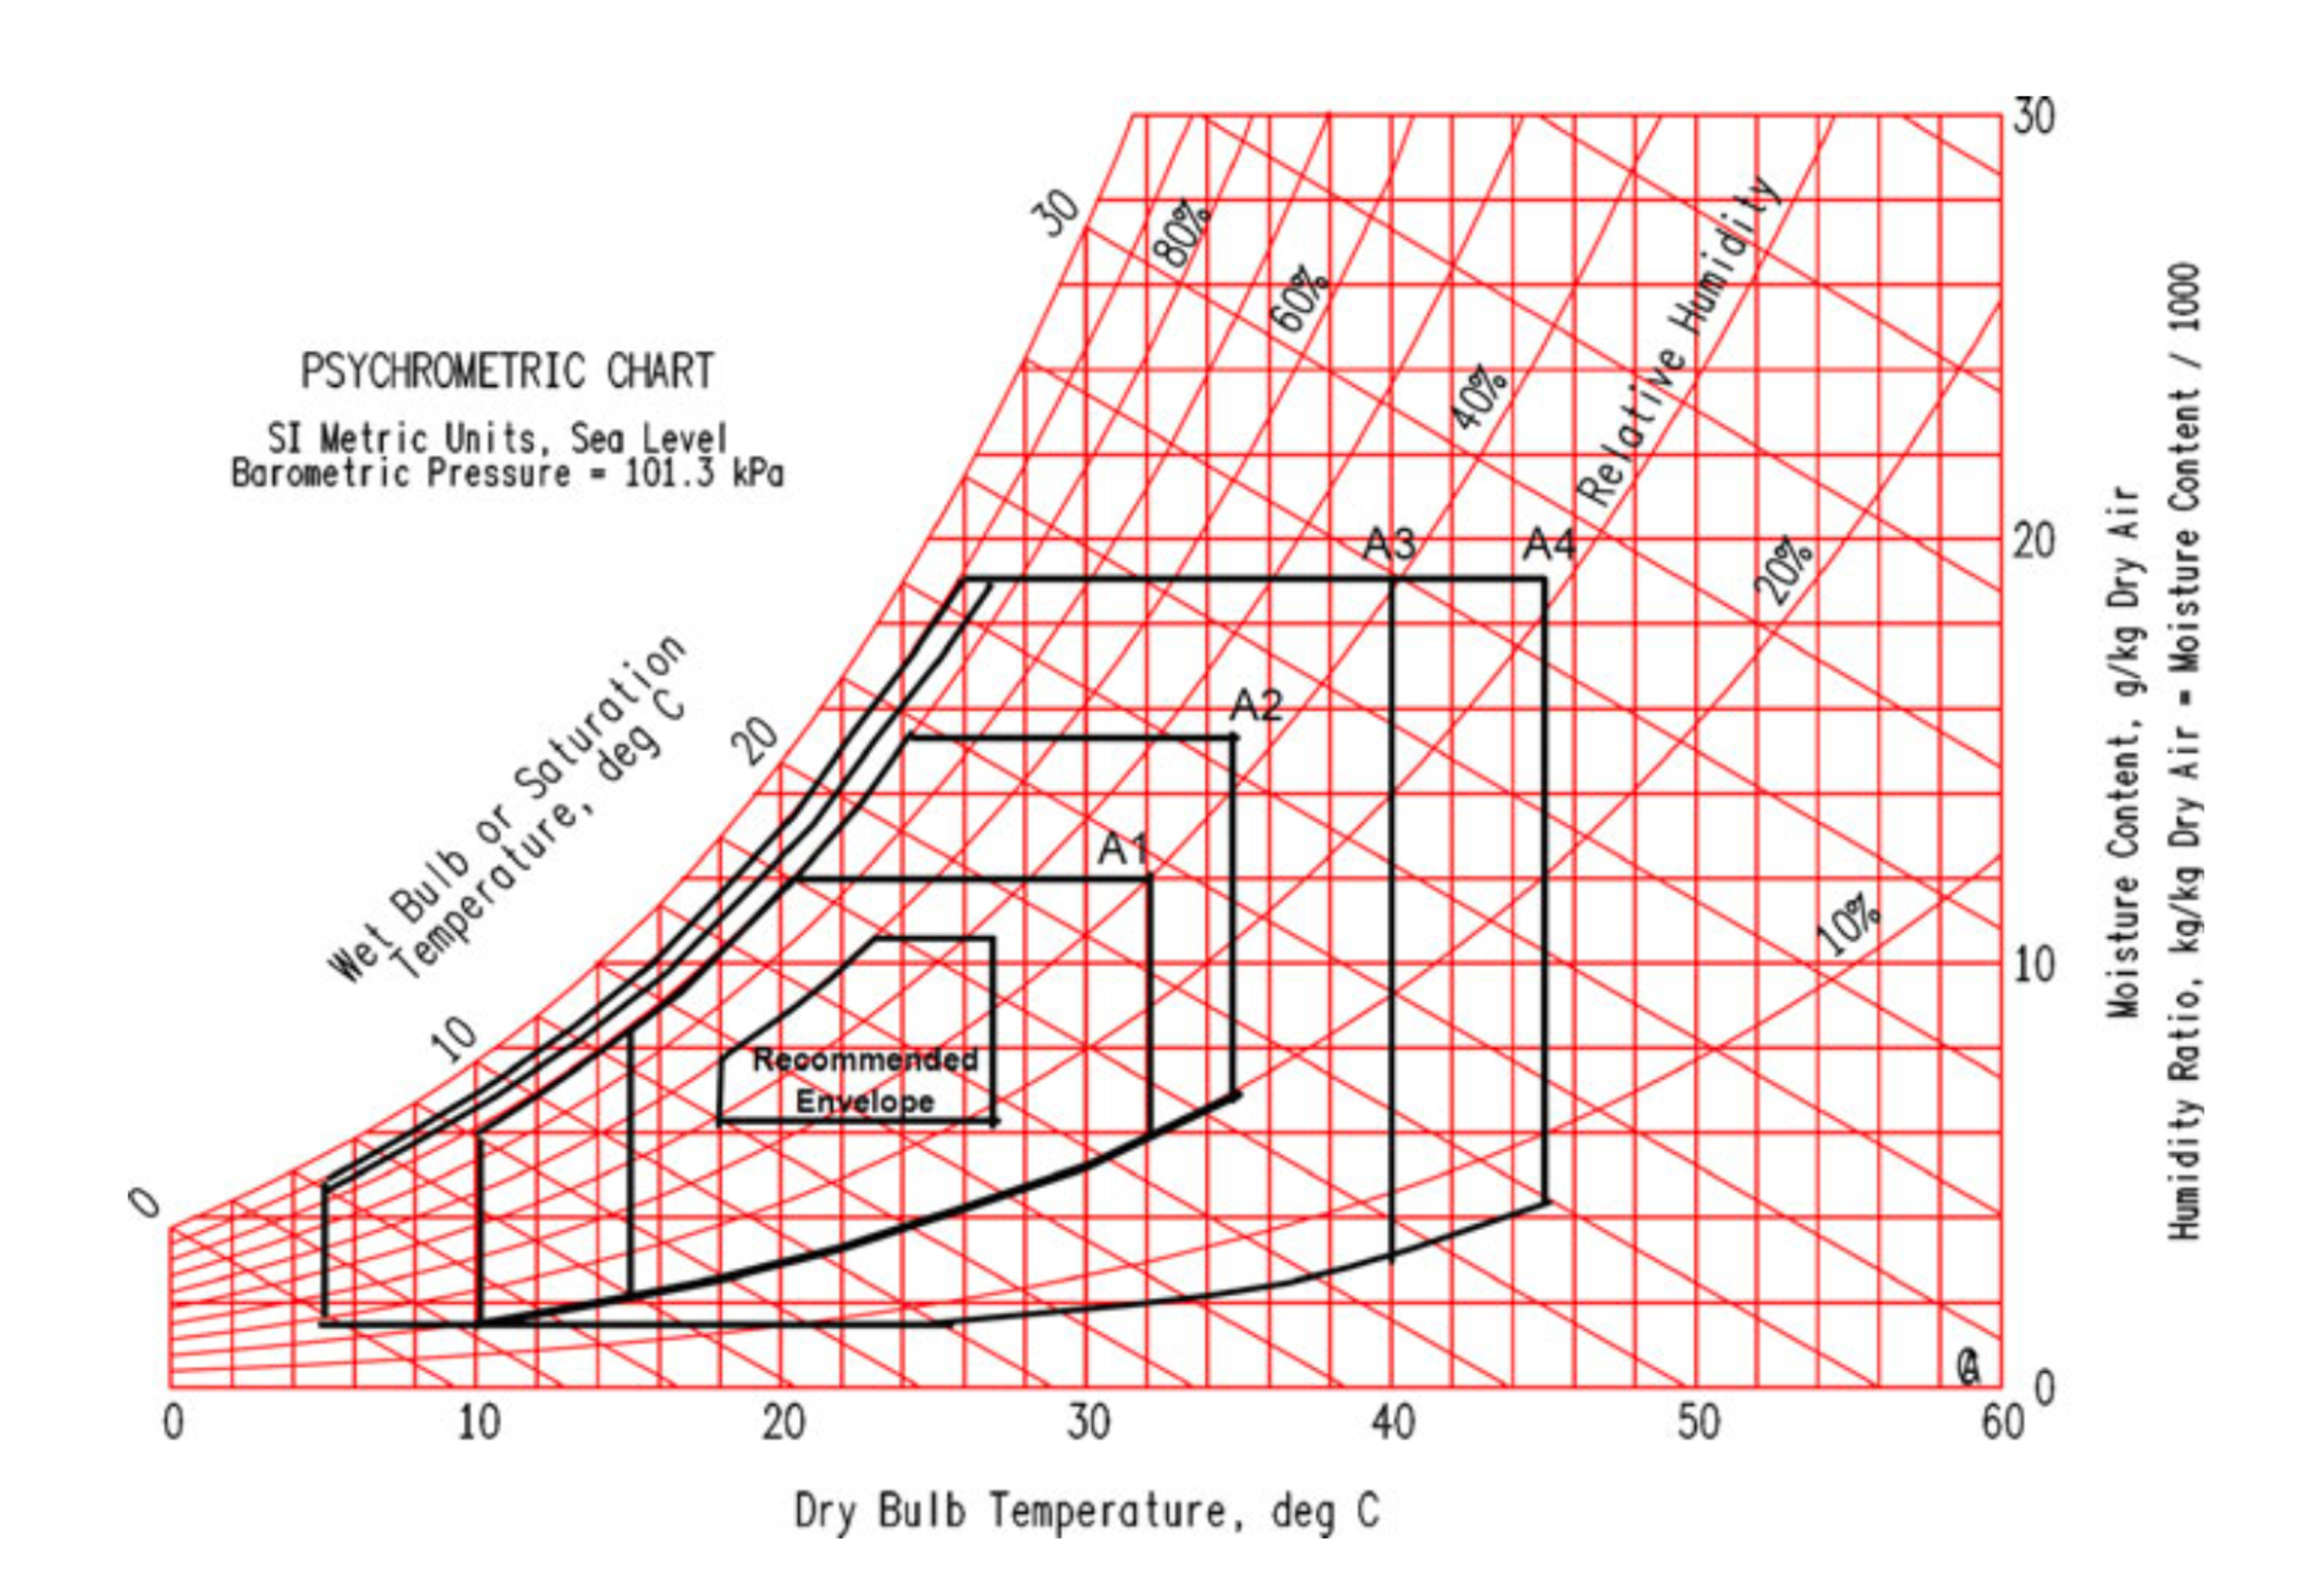
\includegraphics[scale=.3]{methodology/images/psychrometric.eps}
\caption[ASHRAE thermal environment envelope]{ASHRAE thermal environment envelope. Inlet air temperature of IT equipment (\textcopyright 2011 ASHRAE).  Image from \cite{joshi12}}
\label{psychrometric}
\end{figure}
    
    A facility's thermal environment is directly couples the IT and building systems. The first order impacts of this coupling are on the cooling system; spanning from the cooling tower to the node junctions on the nano-scale transistor junctions. The end to end flow of the heat rejection is shown in Figure~\ref{img_dc_infrastructure}. 
    
    \begin{figure} [!h]
\centering
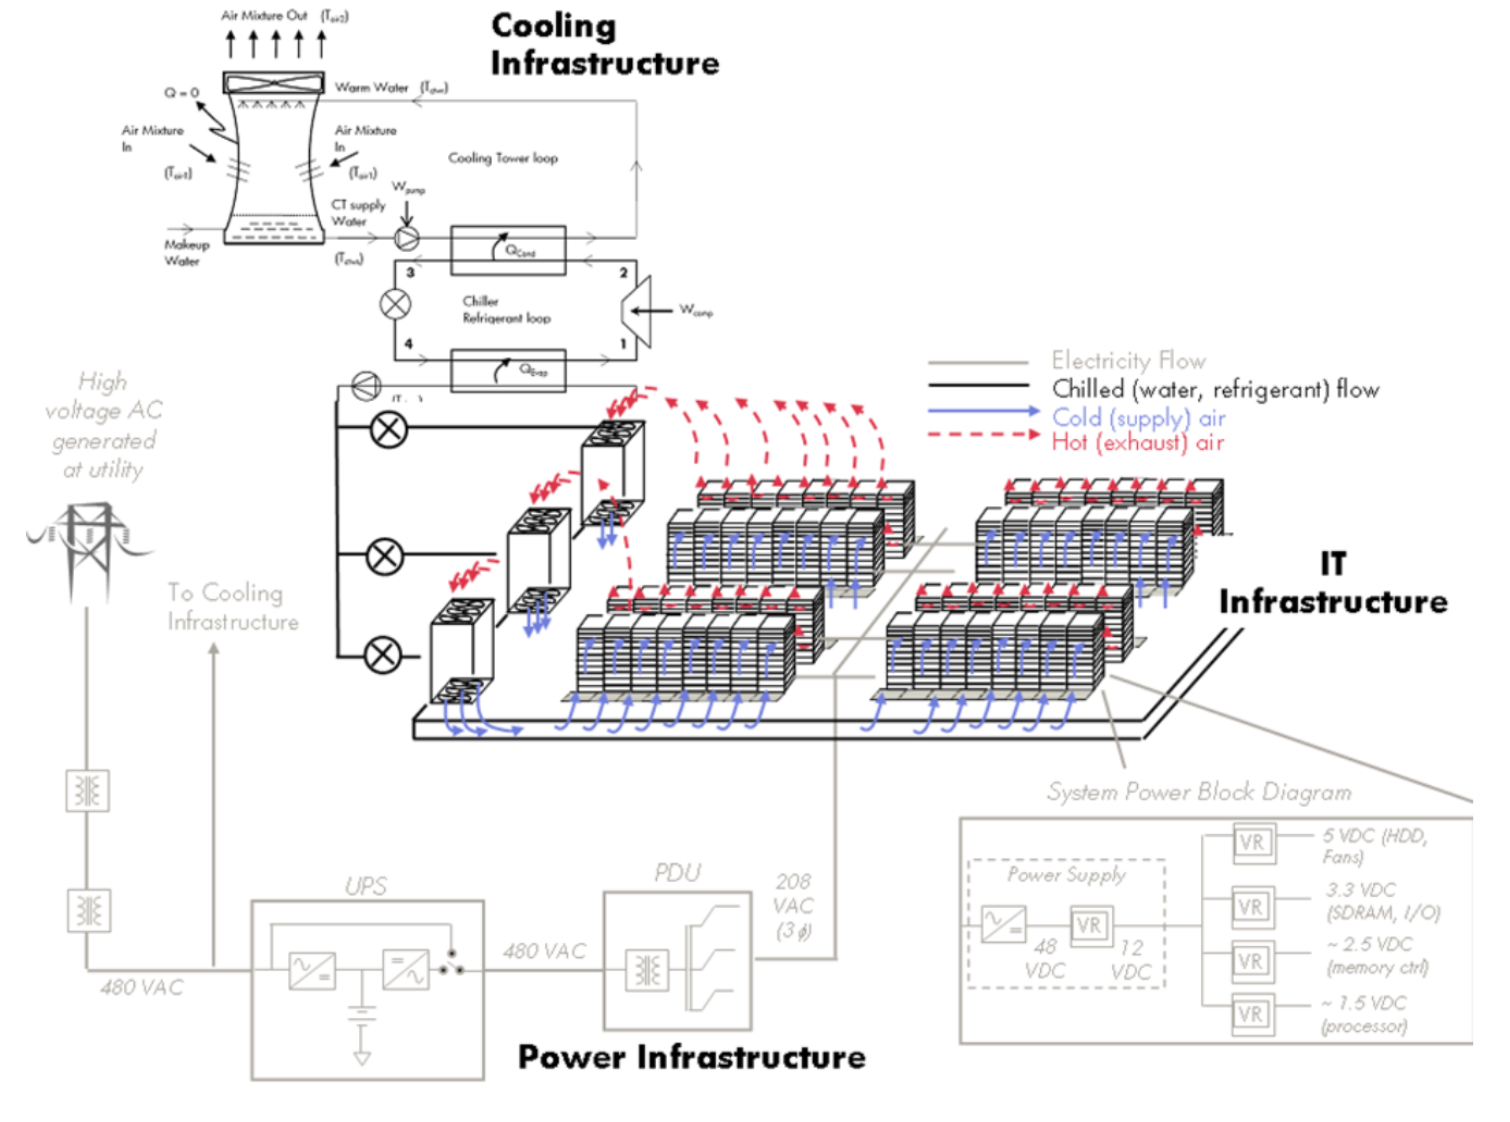
\includegraphics[scale=.25]{methodology/images/dc_cooling.png}
\caption[Image of DC heat rejection paths]{DC Infrastructure Heat Rejection Paths. Image from \cite{shah11}}
\label{img_dc_infrastructure}
\end{figure}
    
    However, there are many second order effects that must me taken into account when developing disruptive designs. For example, one of the undertakings of the researcher that pointed to a life cycle analysis framework was in the development of a novel bottom-cooled hermetic rack \cite{gao16}. The test chamber for the cooling coil and the computational fluid dynamic model of the bottom-cooled rack is shown in \ref{bcu_bench} and \ref{bcu_rack}, respectively. This development alone required a deep trade-off analysis of various systems. 
    
    \begin{figure}[!tbp]
    \subfloat[BCU Air Flow Chamber]{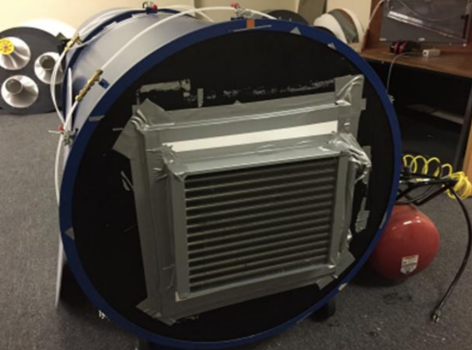
\includegraphics[width=0.35\textwidth]{methodology/images/bcu_airflow_bench.png}
        \label{bcu_bench}}
    \hfill
    \subfloat[BCU Rack]{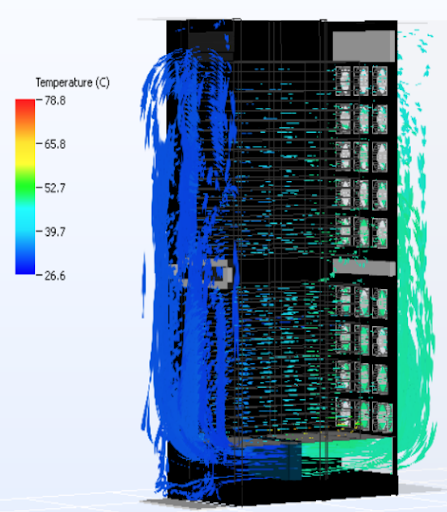
\includegraphics[width=0.4\textwidth]{methodology/images/bcu_rack.png}
        \label{bcu_rack}}
    \caption[Development of Bottom Cooling Units]{Development of Bottom Cooling Units. Image from \cite{gao16}}
\end{figure}
    
    The second order trade offs for such system include the changes required to the building systems, the impacts to the the network topology, chiller plant augments, and power distribution. These trade-offs must be made with awareness of the data center service level agreements as not to strand space, power, or network ports. Furthermore, the business evaluation of such a development efforts must normalize all of the above factors to indicate cost vs. performance to allow consideration of alternate technologies as shown in Figure~\ref{img_bcu_second_order}.
    
    \begin{figure} [!h]
\centering
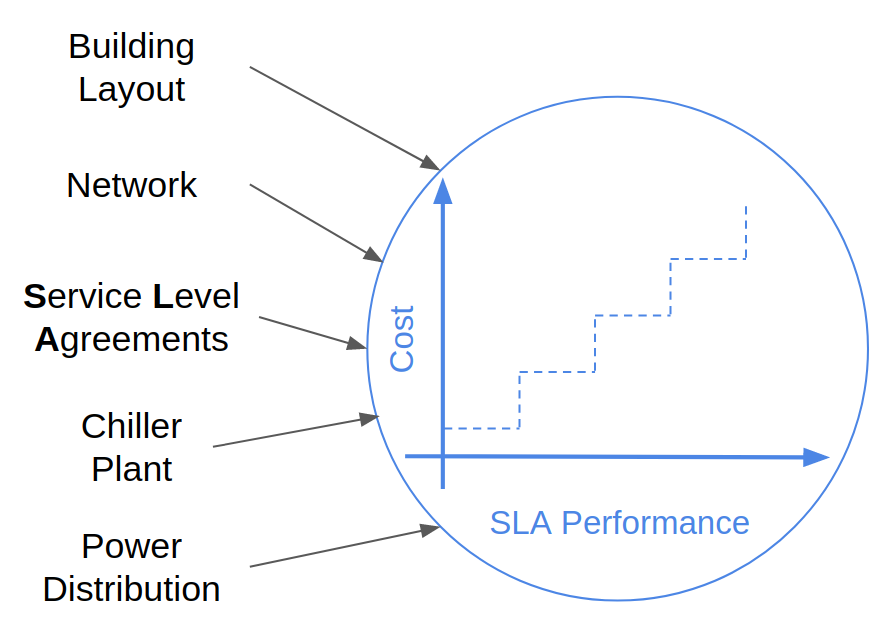
\includegraphics[scale=.25]{methodology/images/bcu_second_order.png}
\caption[Bottom Cooled Unit Second Order Trade-Offs]{Second Order Trade-offs.}
\label{img_bcu_second_order}
\end{figure}
    
    Beyond the operations phase of DCs, the IT hardware and physical infrastructure products they're composed of have many other life-cycle phases. At each life cycle phase of the products there are energy and $CO_2$ inventories. With life cycle analysis (LCA) principles these inventories can be tallied from their raw form to their useful state.  The LCA perspective allows the treatment of these inventories as either a debt or credit to it's environmental footprint. The debt and credit approach follows a structure analogous to total costs of ownership (TCO) methods used in today's sophisticated business models for DCs. These modern business models amortize capital and operating costs over a system's useful life similar to LCA. This research therefore threats $CO_2$ as analogous to monetary cost and demonstrates the end to end $CO_2$ inventories in this dissertation.
    
    The direct effects described so far and discussed throughout this work are the most transparent impacts associated with information communication technology (ICT). The indirect or higher order impacts fundamentally alter the use of energy in a wide breadth of applications. Figure~\ref{ICT_econ} shows examples of the breadth ICT impacts to other industrial sectors. However, this research followed the approach set by The Green Grid where the DC is a physical entity of interest and focuses on the assessment of it's direct life cycle activities \cite{tgg12}. The direct activities are indicated by the red boundary shown in figure  \ref{fig:f2} which sets the boundary conditions described later. 
    
    
\begin{figure}[!tbp]
    \subfloat[Influence and Impacts of ICT to other sectors]{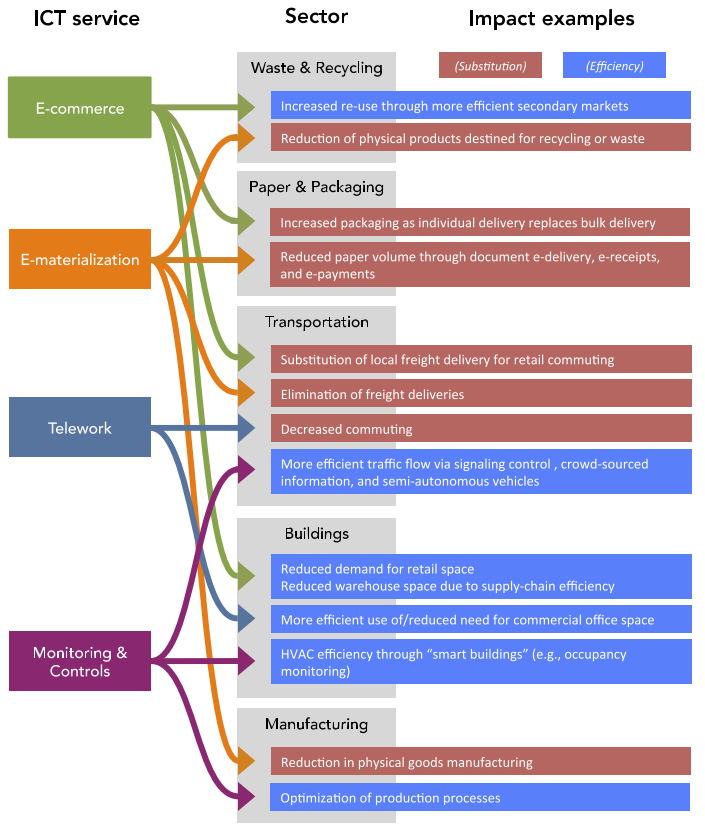
\includegraphics[width=0.5\textwidth]{methodology/images/ICT_econsec.png}
        \label{ICT_econ}}
    \hfill
    \subfloat[Taxonomy of ICT impacts]{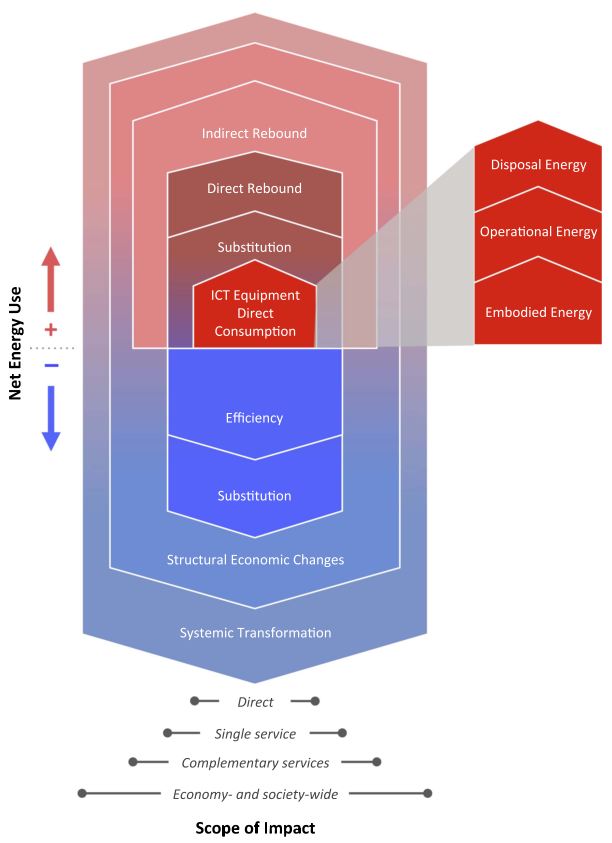
\includegraphics[width=0.4\textwidth]{methodology/images/ICT_scopes.png}
        \label{fig:f2}}
    \caption[Higher Order ICT Impacts]{Higher Order ICT Impacts. Images from \cite{Horner16b}}
\end{figure}
    
\section{Similar Literature}
    
    Now, pioneering literature to quantify the life cycle costs of DCs is presented. The most explicit DC life cycle costs is by Whitehead \cite{whitehead15}. Whitehead proposes guidelines and criterion for DC life cycle assessments in-line with ISO 14040 \cite{ISO14040}. These ISO standards are the authoritative standard for Life Cycle Assessment (LCA) work.  Whitehead's work is based on the LCA of a UK DC with legacy infrastructure. The UK DC is compared to a state of the art DC in Sweden across all phases of their life cycle. The boundary conditions and life cycle phases from Whitehead are shown in figure \ref{LCAphases}. Through sensitivity analysis, Whitehead finds that server stock turnover (refresh) cycles have  the most significant contribution to the embodied impacts in today's state of the art DCs.  Embodied impacts for these DCs dominate the life cycle impacts even more so as the state of the art DCs are optimized for PUE with efficient cooling and power distribution systems . To demonstrate, they performed a comparative evaluation. When quantified, the environmental impacts were double for the Swedish facility. Whitehead attributes this difference to the Swedish data refresh cycle of every 16 months, as opposed to every 36 months for the UK DC. They establish a functional unit of \textit{1 kW of IT per year in a Tier III facility} which is a reasonable units of measure of data centers.
    
    \begin{figure} [!h]
\centering
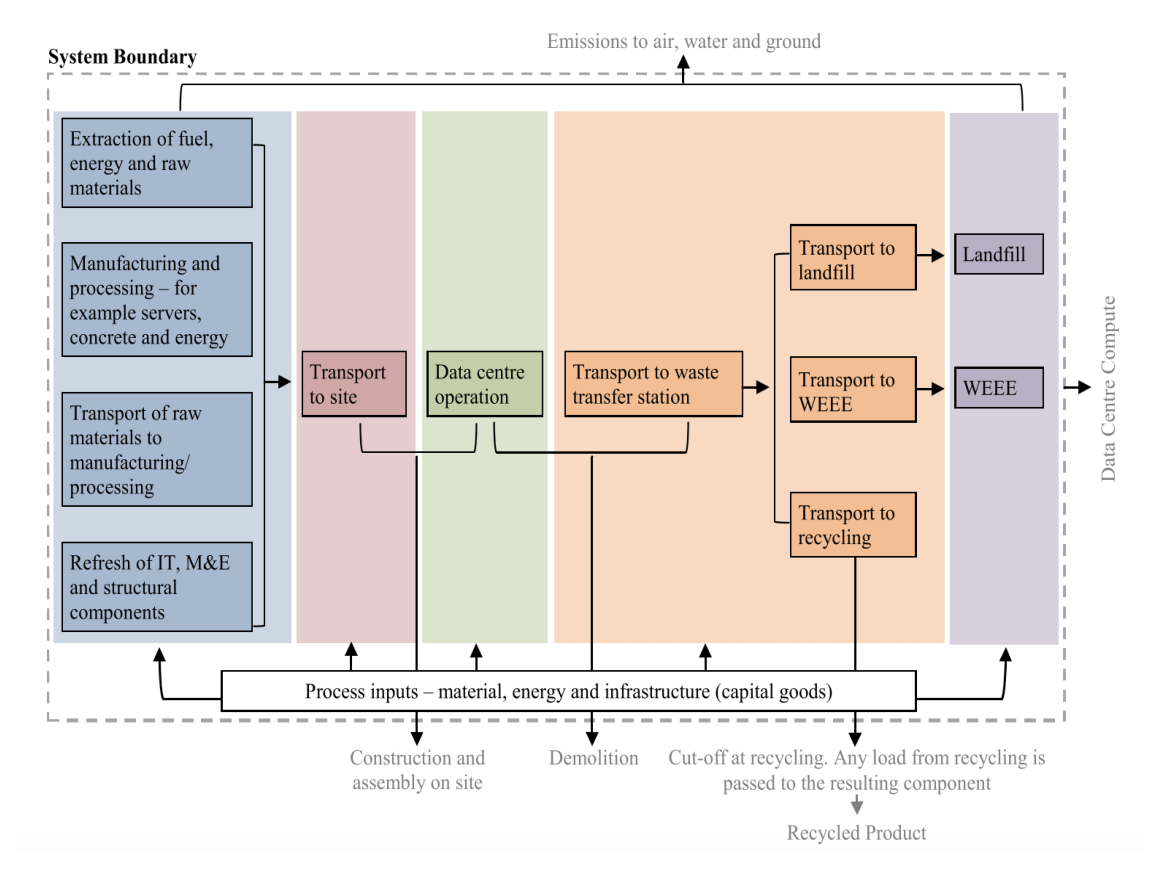
\includegraphics[scale=.6]{methodology/images/LCAphases.eps}
\caption[Whitehead DC LCA Boundary]{System boundary for DCs. Image from \cite{whitehead15}}
\label{LCAphases}
\end{figure}
    
    The Hewlett Packard Corporation published a series of papers around the sustainability of information technology sector in the early 2010's. Two of the most relevant to data centers were led by Shah and Chang \cite{shah11, shah12}. In the first work, Shah demonstrated the use of the economic input-output (EIO) model for assessing the embodied costs of the major infrastructure categories found in data-centers (see Table \ref{shah_components}). Their development of the environmental model for the data center was ultimately a combination of process based and EIO methods. Building on Shahs's EIO based framework, Chang uses the thermodynamic metric of exergy to quantify data center sustainability. By quantifying the irreversible thermodynamic processes in terms of exergy allows normalization in terms of architectural parameters \cite{shah12}. A parametric view enables systems designers to reason about only an intuitive set of constraints.
    
    \begin{table}[h!]
    \begin{center}
    \scalebox{0.6}{
    \pgfplotstabletypeset[
        col sep=comma,
        string type,
        every head row/.style={before row=\hline,after row=\hline\hline},
        every last row/.style={after row=\hline},
        ]{methodology/content/data/shah_boundaries.csv}}
    \end{center}
    \caption{Components considered by Shah \cite{shah11}
}    \label{shah_components}
\end{table}

    
    In addition to the independent LCA perspective of Whitehead and the corporate perspective of Hewlett Packard, The Department of Energy's Lawrence Berkeley National Lab  has produced the CLEER online modeling tool\cite{CLEER13}. CLEER is a web based user interface that allows consumers to model the migration of the CLEER model to assess the life cycle cost of migrating on-premise software workloads to Cloud based data center platforms. As shown in Figure~\ref{img_cleer}, the charter for the CLEER model to consider the end to end energy associated with Cloud services.
    
    \begin{figure} [!h]
\centering
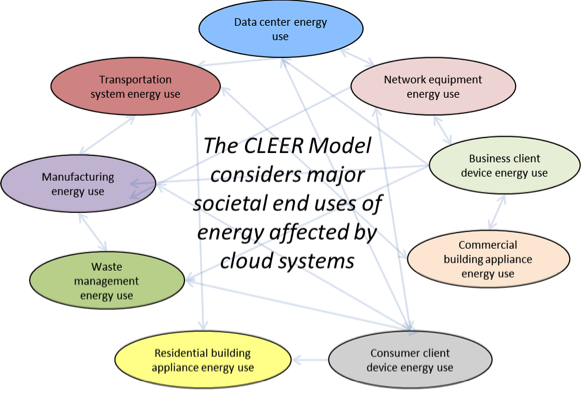
\includegraphics[scale=.5]{methodology/images/cleer_diagram.png}
\caption[CLEER Framework]{CLEER Framework.  Image from \cite{CLEER13}}
\label{img_cleer}
\end{figure}
    
    In the subsequent chapters, this research builds upon these pioneering similar works. Six parameters common to all three are identified and supplemented with novel contributions developed by this dissertations research. Two additional are also added to make the end to end modeling framework presented dynamic in terms of network traffic and building operations as shown in Figure~\ref{img_gap_matrix}
    
    \begin{figure} [!h]
\centering
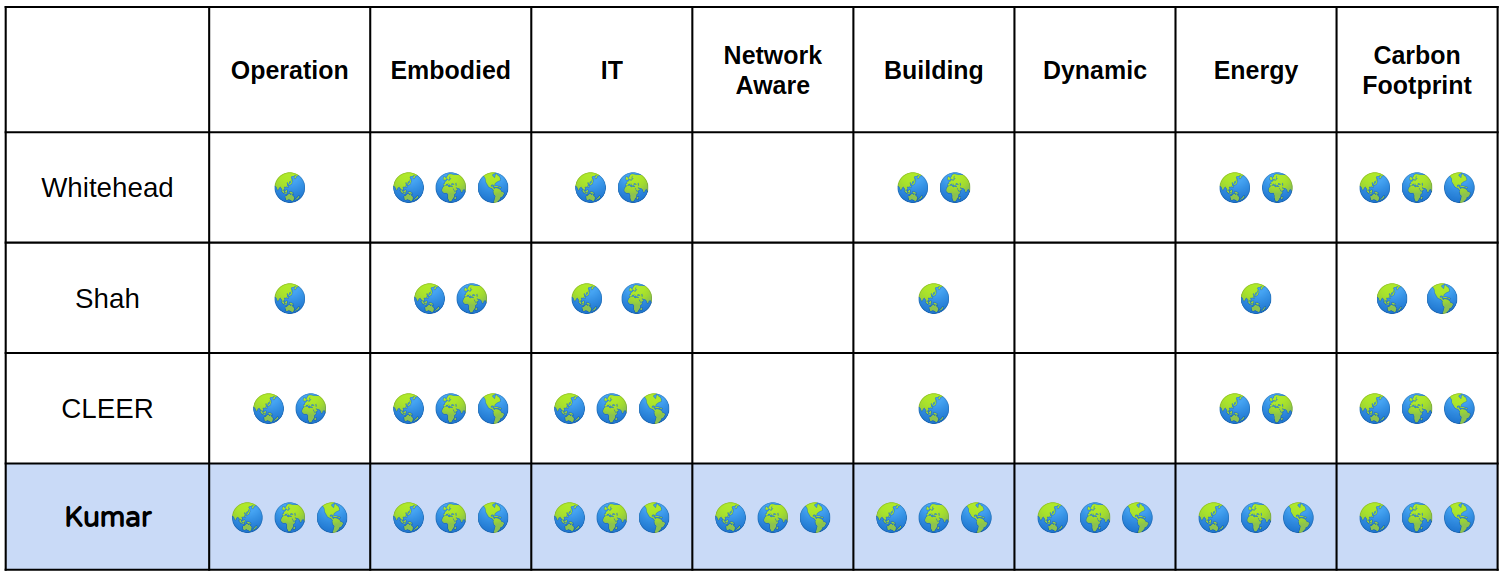
\includegraphics[scale=.25]{methodology/images/gap_matrix.png}
\caption[Research Gap Matrix]{Gap Matrix.}
\label{img_gap_matrix}
\end{figure}
    
    In this section the background discussed has inspired the research question pursued in the dissertations. Namely the research question is; how can DC design decisions that have longevity  with all of the uncertainty involved? Next the research hypothesis is stated followed by and overview of the specific methods that are used to validate the hypothesis.
    
\section{Hypothesis}

    \emph{To make effective DC design capacity decisions, the decisions must be based on scalable and agile models.} 
        
    Sub hypothesis are as follows:
    
    \begin{enumerate}
        \item The model needs to assess end to end cost trade-offs and be technology agnostic.
    
        \item Monetary cost models for DCs are analogous to environmental cost models. LCA modeling community has proven its effectiveness for analysing global scale systems and supply chains.
    \end{enumerate}
    
\section{Structure of Dissertation}

    This research is composed of four modules that culminate academic desktop analysis and extensive extensive professional experiences with designing, planning, building, and deploying data center system through out the world. The modules are presented in this dissertation as independent, but correlated chapters. The segmentation of the chapters roughly aligns with the the software modules developed as shown in Figure~\ref{process_flow}.
    
    \begin{figure}[h]
\centering
\begin{tikzpicture}
\node [anchor=west] (scope) at (8.75,5.5) {Embodied Costs};
\node [anchor=west] (traffic) at (1.4,5.5) {Traffic};
\node [anchor=west] (bem) at (4.2,5.5) {BEM};
\node [anchor=west] (mec) at (6.75,5.5) {MEC};
\begin{scope}[xshift=1.5cm]
    \node[anchor=south west,inner sep=0] (image) at (0,0) {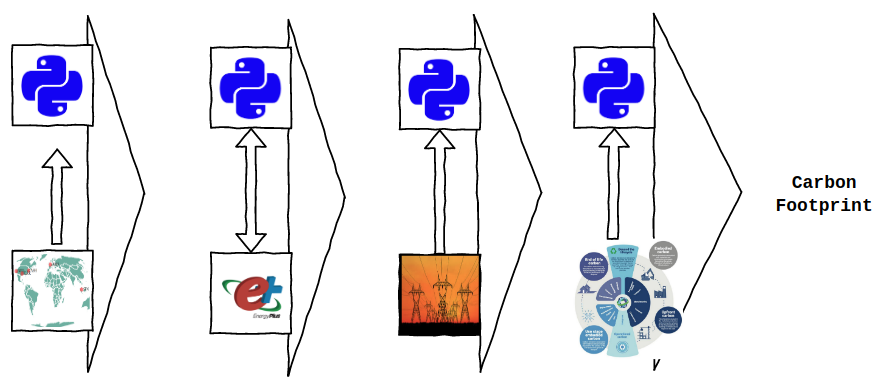
\includegraphics[width=0.8\textwidth]{embodied_cost_model/images/horizontal_process_flow.png}};
    \begin{scope}[x={(image.south east)},y={(image.north west)}]
        % \draw[ultra thick,rounded corners, ,dashed] (0.625,1.0) rectangle (0.85,0.0);
        % \draw [-stealth, line width=5pt, cyan] (scope) -- ++(0.6,0.0);
    \end{scope}
\end{scope}
\end{tikzpicture}
\caption[Model Process Flow Diagram]{Model Process Flow Diagram.}
\label{process_flow}
\end{figure}

\section{Data sources and overview of the targeted data center systems design.}
    The under laying data that constructs and validates the developed software modules are sourced from publicly available references and professional heuristics. Generally, the preference of this research is to use publicly available data for academic posterity, however there are several critical pieces of information that are not publicly available. In these cases, where no relevant public information was found, the author leans on heuristics. Due to the nature of the technology business, most of the heuristically derived data points are protected under non disclosure agreements, and are presented in generalized terms where meaning is not lost. In cases where generalization leads to misconstruing the data, any indicator pointing to specific business organizations is striped out. 
    
\section{Information Technology Equipment}
        The modeling framework developed in this research requires details about the information technology hardware from inside the data centers. Low fidelity representations of the hardware configurations suffice for the building energy and EIO based embodied materials modules. Table~\ref{computer_parts} indicates the data used in this research to characterize the information technology hardware. This data is based on production server configurations of a large internet operator, representing their deployments in 2015 and 2016. 
        
        By nature of the technology sector, the server configurations have a high temporal sensitive; as new products and optimizations are brought to market on quarterly cadences that pivot the total costs of ownership models. Figure shows air cooled server units fitted with a combination of processors and  
        
        \begin{figure} [!h]
\centering
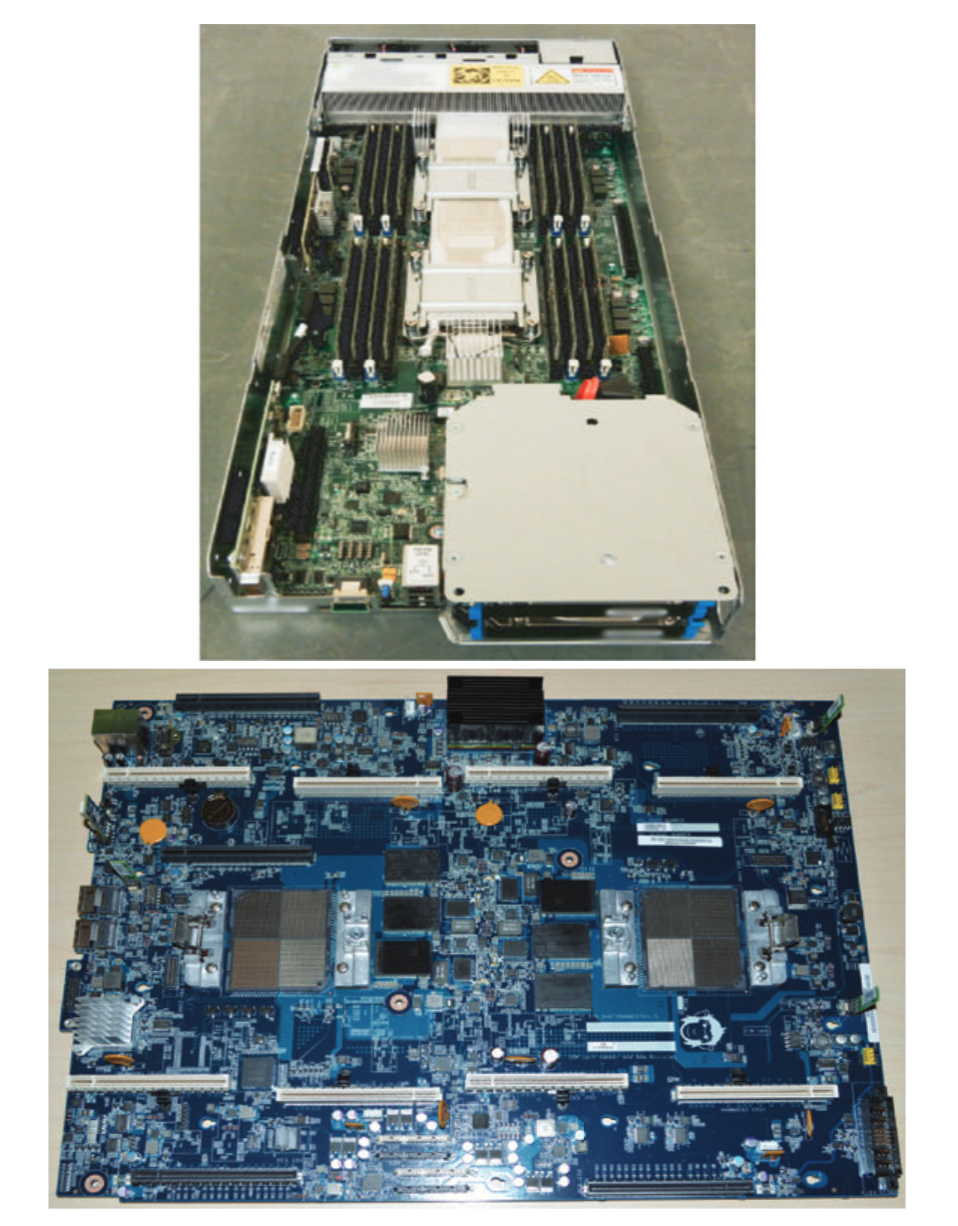
\includegraphics[scale=.5]{methodology/images/server_image.png}
\caption[Barroso's Servers]{(Top) Intel Haswell-based server tray and (Bottom) IBM Pow-er8-based server tray.  Images from \cite{barroso13}}
\label{img_server}
\end{figure}
        
        In this work, a combination of server components from Table~\ref{computer_parts} are aggregated based on the total power of the building using Algorithm~ \ref{it_y_vector_algo}. This is sufficient for building design tasks and in practice this is the granularity that facilities stake holders handle. Finer granularity is not sought as the models that are developed in this research don't optimize or even account for the air flow patterns or equipment layout inside the buildings. Nonetheless the fidelity of the framework can be enhanced for quantifying the operational energy and embodied materials if the physical layouts of the servers and buildings are more precisely characterised.
        
        \begin{table}[h!]
    \begin{center}
    \scalebox{0.5}{
    \pgfplotstabletypeset[
        col sep=comma,
        string type,
        every head row/.style={before row=\hline,after row=\hline\hline},
        every last row/.style={after row=\hline},
        ]{methodology/content/data/Server_Component_Counts.csv}}
    \end{center}
    \caption[Server types and components used in modeling]{Server types and components within these servers modeled in the simulations performed for this research.}
    \label{computer_parts}
\end{table}
        
        %  Examples of the design choices for the server components arrangements and building layouts are now discussed. These examples point to modeling improvements that can make this framework more precise. Furthermore, these example are used to normalize the servers into their deploy-able units; a server rack.
        
        Steel racks host the server assemblies. Figure~\ref{bcu_rack} and Figure~\ref{goog_rack} are examples of hyper-scale racks. There are several design paradigms for combining various components with the racks. Design choices range from fully homogeneous racks to 
        
        \begin{figure} [!h]
\centering
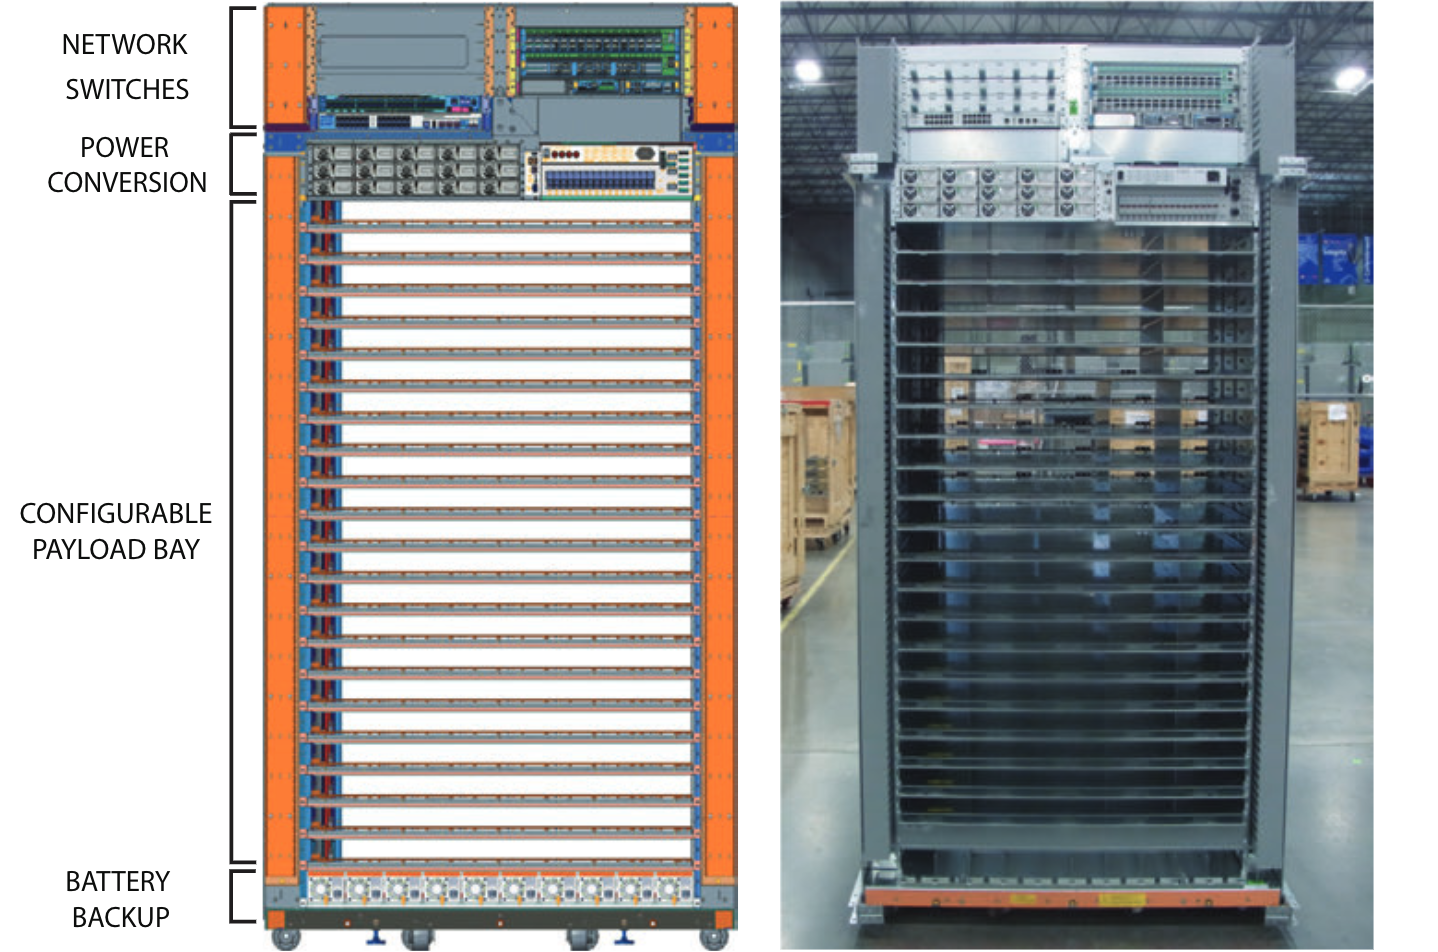
\includegraphics[scale=.5]{methodology/images/goog_rack.png}
\caption[Example Server Rack]{Server rack with top of rack switch, power shelf, server trays slots, and local batteries. Image from \cite{barroso18}}
\label{goog_rack}
\end{figure}
        
        Network - Top of Rack Switch
        Rectifiers - 
        Servers
    
        \subsubsection{Network Model}
    
        \subsubsection{Building Systems}
        
        The the form factor of data center facilities is heavily influenced by the mechanical systems conveying heat from the racks a heat sink. Figure~\ref{img_airflow} illustrates the airflow path across a data center from the point that air enters the building until it is exhausted.
        
        \begin{figure} [!h]
\centering
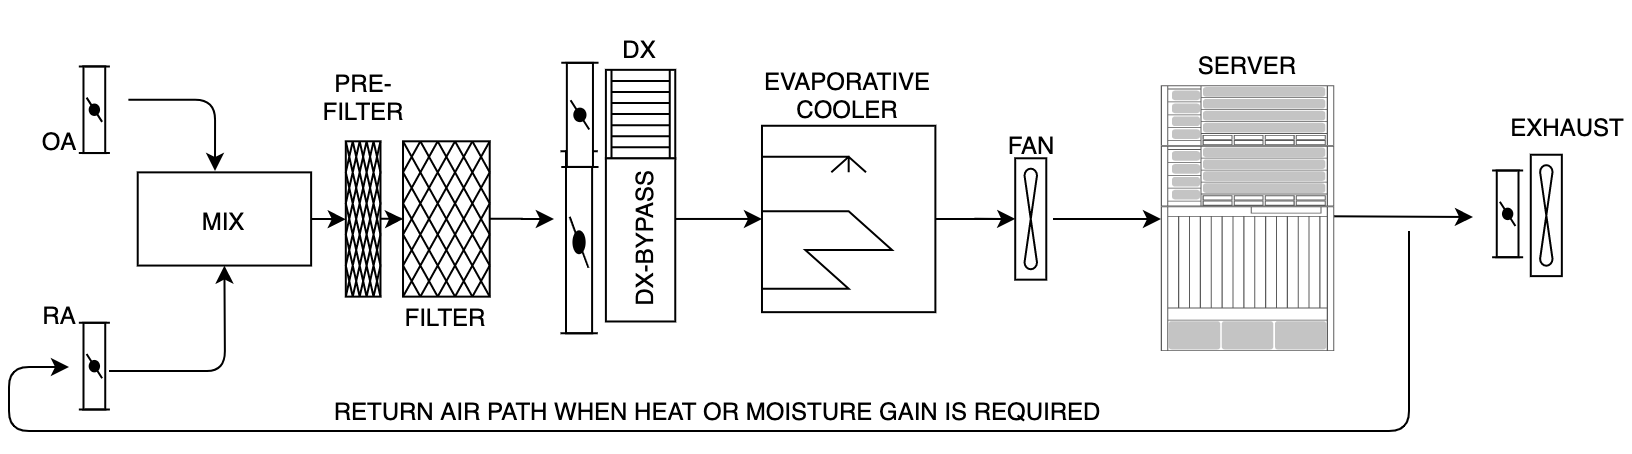
\includegraphics[scale=.5]{methodology/images/airflow.png}
\caption[Airflow through DCS]{Generic air flow path in server rooms for an outside air cooled facility.}
\label{img_airflow}
\end{figure}
        
        \subsubsection{Marginal Cost of Energy}
    
   
    

    
    
